\section{Exercise three}

Consider the C program below:
\begin{verbnobox}[\verbarg]
#include <stdio.h>
#include <stdlib.h>
#include <string.h>

void vuln(int n) {
        struct {
        char buf[16];
        char tmp[16];
        int sparrow = 0xBAAAAAAD;
    } s;

    if (n > 0 && n < 16) {
        fgets(s.buf,n,stdin);
    if(strncmp(s.buf, "H4CK", 4) != 0 && s.buf[14] != “X”) {
        abort();
    }
    scanf("%s", s.tmp);
    if(s.sparrow != 0xBAAAAAAD) {
        printf("Goodbye!\n");
        abort();
        }
    }
}

int main(int argc, char** argv) {
    vuln(argc);
    return 0;
}  
\end{verbnobox}
\begin{enumerate}
    \item Assume the usual IA-32 architecture (32-bits), with the usual \texttt{cdecl} calling convention. 
    Assume that the program is compiled without any mitigation against exploitation (the address space layout is not randomized, the stack is executable, and there are no stack canaries).
    Draw the stack layout when the program is executing the instruction at line twelve, showing:
    \begin{itemize}
        \item Direction of growth and high-low addresses.
        \item The name of each allocated variable.
        \item The boundaries of frame of the function frames (\texttt{main} and \texttt{vuln}).
    \end{itemize}
    Show also the content of the caller frame (you can ignore the environment variables, just focus on what matters for the vulnerability and its exploitation).
    \item The program is affected by a typical buffer overflow. 
        Find the line affected and describe the reason. 
    \item Write an exploit for the buffer overflow vulnerability in the above program to execute the following simple shell code, composed only by four instructions: \texttt{0x51 0x52 0x5a 0x5b}. 
        Make sure that you show how the exploit will appear in the process memory with respect to the stack layout right before and after the execution of the detected vulnerable line during the program exploitation. 
        Ensure you include all of the steps of the exploit, ensuring that the program and the exploit execute successfully. 
        Include also any assumption on how you must call the program (e.g., the values for the command-line arguments required to trigger the exploit correctly, environment variables).
    \item Let's assume that the C standard library is loaded at a known address during every execution of the program, and
    that the (exact) address of the function \texttt{system()} is \texttt{0xf7e38da0}. 
        Explain how you can exploit the buffer overflow vulnerability to launch the program \texttt{/bin/secret}.
    \item Assume now that the program is compiled without any mitigation against exploitation (the address space layout is not randomized, the stack is executable, and there are no stack canaries). 
    Propose the simplest modification to the C code provided that solves the buffer overflow vulnerability detected, motivating your answer. 
\end{enumerate}

\subsection*{Solution}
\begin{enumerate}
    \item Notice that the elements of the \texttt{struct} are stacked in reverse order. 
        Therefore, the stack's structure at line twelve is as depicted below:
        \begin{figure}[H]
            \centering
            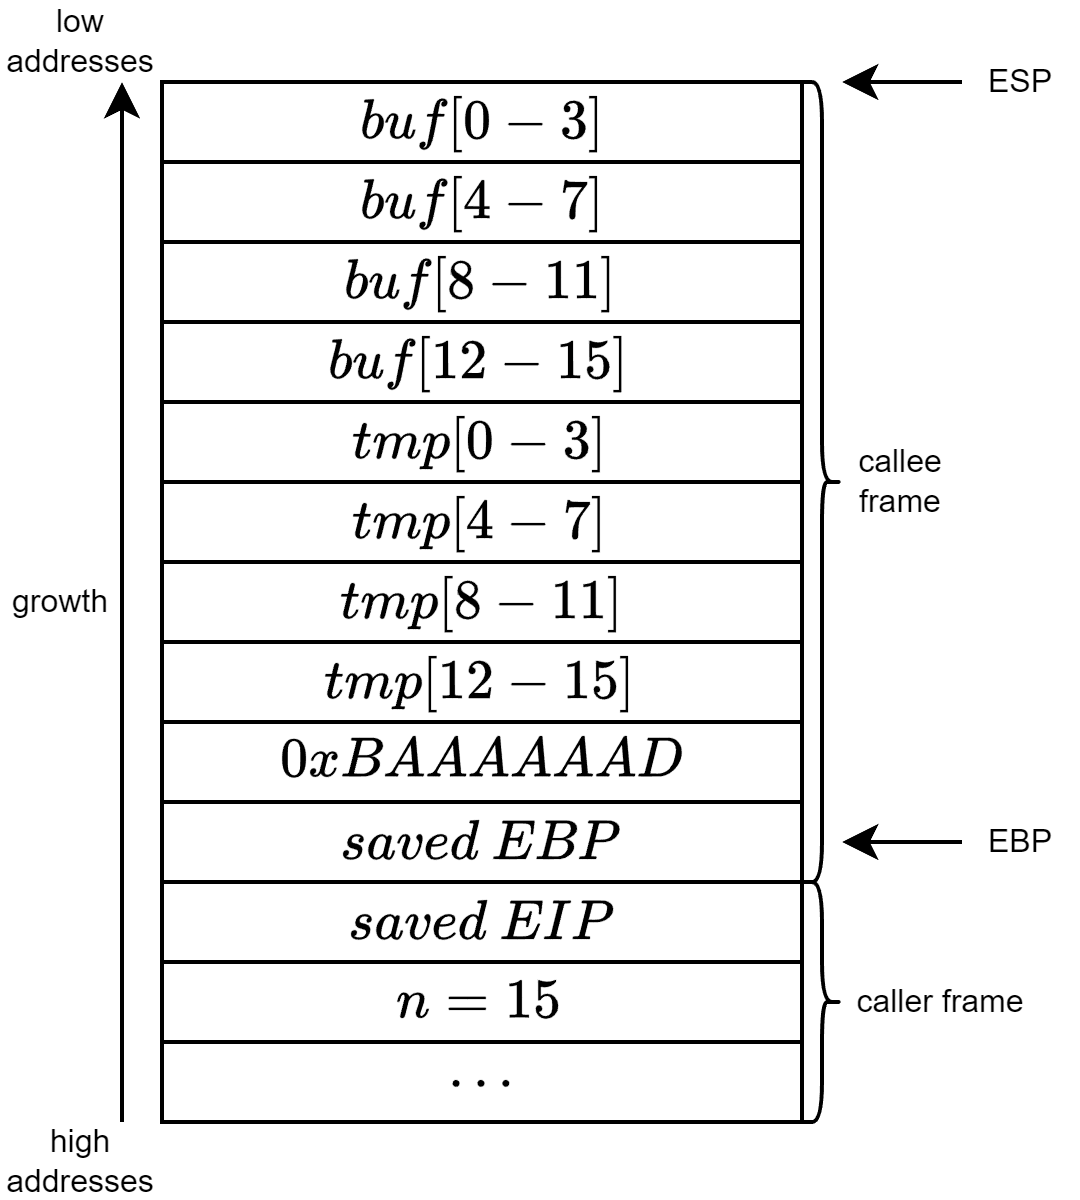
\includegraphics[width=0.5\linewidth]{images/stack3.png}
        \end{figure}
    \item The buffer overflow occurs at line seventeen because \texttt{scanf} reads an entire string without considering the size of the \texttt{buf} buffer. 
        Conversely, at line thirteen, there's no buffer overflow since the value of $n$ is guaranteed to be smaller than the buffer's size.
    \item The exploit can be executed with the following stack modification:
        \begin{figure}[H]
            \centering
            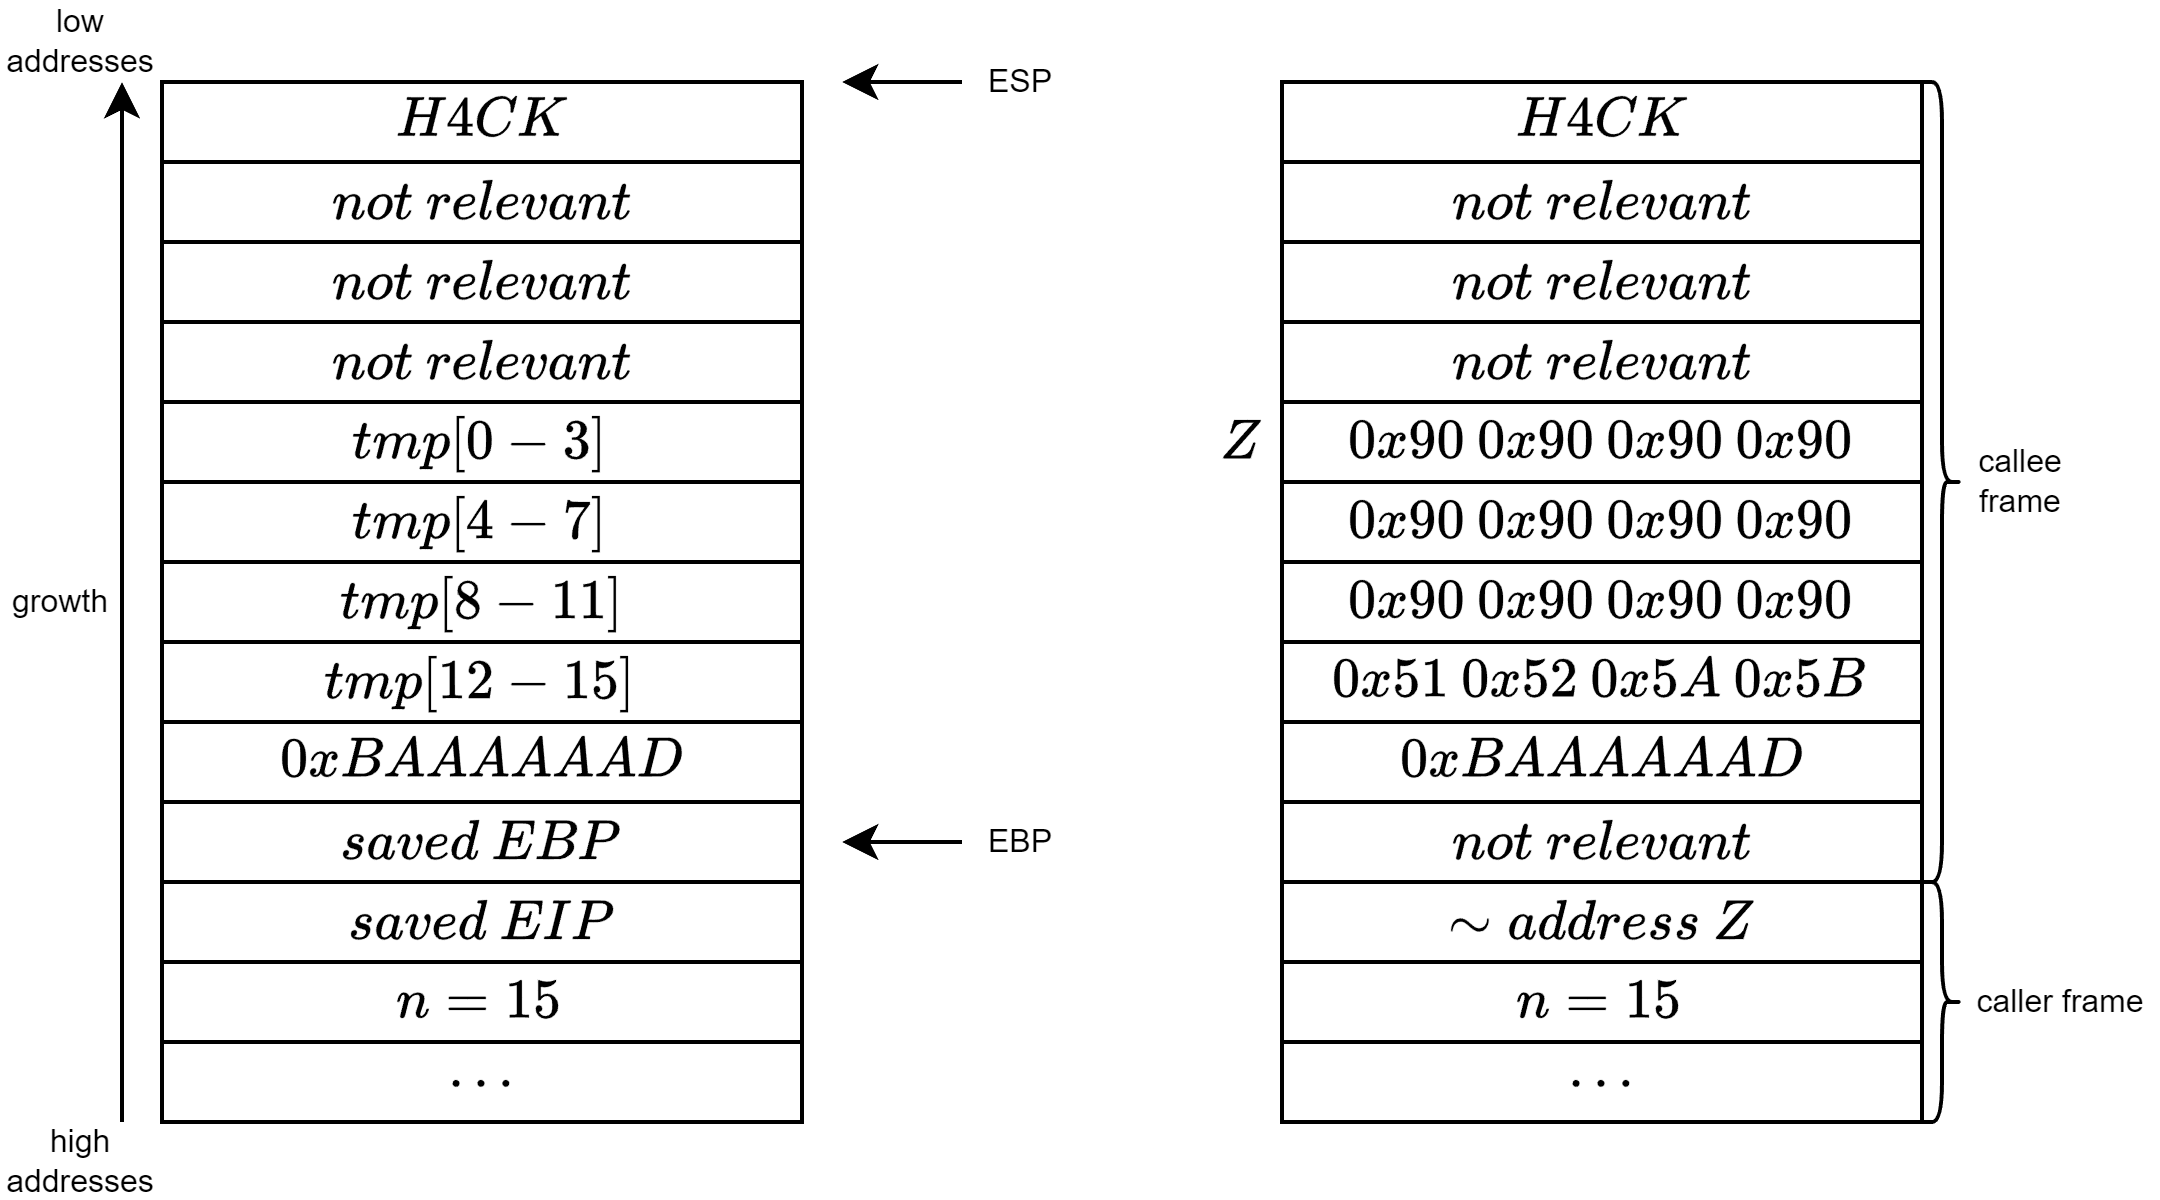
\includegraphics[width=0.75\linewidth]{images/stack4.png}
        \end{figure}
    \item We first write the string \texttt{/bin/secret} into \texttt{tmp} and then overwrite the saved EIP with the address of \texttt{system()}. 
        Subsequently, we overwrite an additional 8 bytes for the \texttt{system()} EIP and for the pointer to \texttt{Y}. 
        This ensures that upon jumping into the \texttt{system()} function, the pointer will be correctly positioned for \texttt{system()} to execute with the expected parameters.
    \begin{figure}[H]
            \centering
            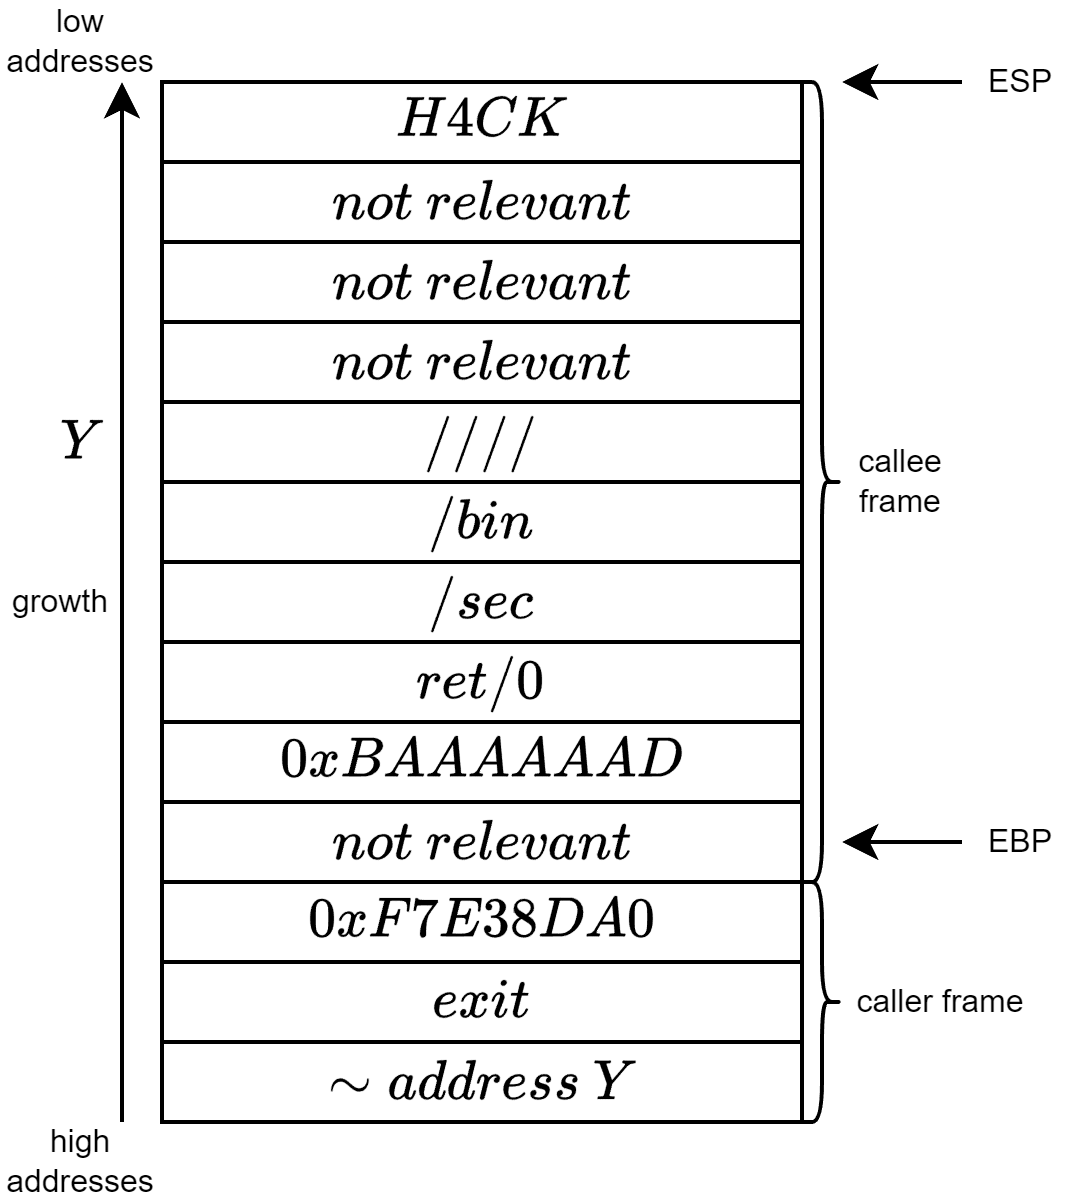
\includegraphics[width=0.5\linewidth]{images/stack5.png}
        \end{figure}
    \item To address the vulnerability, the line can be rewritten in one of the following ways:
        \begin{verbatim}
scanf("%15s", s.tmp);
fgets(s.tmp,15,stdin);
        \end{verbatim}
\end{enumerate}